\documentclass[runningheads,a4paper]{llncs}
\usepackage[T1]{fontenc}
\usepackage{amsmath,amssymb}
\usepackage{graphicx}
\usepackage{booktabs}
\usepackage{array}
\usepackage{lmodern}
\usepackage[expansion=false]{microtype}
\usepackage{tikz}

\renewcommand{\topfraction}{.95}\renewcommand{\bottomfraction}{.90}\renewcommand{\textfraction}{.05}\renewcommand{\floatpagefraction}{.85}
\setlength{\textfloatsep}{4pt plus 1pt minus 1pt}
\setlength{\floatsep}{3pt plus 1pt minus 1pt}
\setlength{\intextsep}{3pt plus 1pt minus 1pt}
\setlength{\abovecaptionskip}{2pt}
\setlength{\belowcaptionskip}{0pt}
\makeatletter
\renewcommand\section{\@startsection{section}{1}{\z@}%
                       {-6\p@ \@plus -1\p@ \@minus -1\p@}%
                       {3\p@ \@plus 1\p@ \@minus 1\p@}%
                       {\normalfont\large\bfseries\boldmath
                        \rightskip=\z@ \@plus 8em\pretolerance=10000 }}
\renewcommand\subsection{\@startsection{subsection}{2}{\z@}%
                          {-5\p@ \@plus -1\p@ \@minus -1\p@}%
                          {2\p@ \@plus 1\p@ \@minus 1\p@}%
                          {\normalfont\normalsize\bfseries\boldmath
                           \rightskip=\z@ \@plus 8em\pretolerance=10000 }}
\renewcommand\paragraph{\@startsection{paragraph}{4}{\z@}%
                         {3\p@ \@plus 1\p@ \@minus 1\p@}%
                         {-0.5em}%
                         {\normalfont\normalsize\bfseries}}
\makeatother
\usetikzlibrary{arrows.meta,positioning,fit,backgrounds}
\emergencystretch=2em
\setlength{\tabcolsep}{3pt}

\usepackage{array}
\newcolumntype{L}[1]{>{\raggedright\arraybackslash}p{#1}}
\newcommand{\Msplit}{M_{\mathrm{split}}}
\newcommand{\Munified}{M_{\mathrm{unified}}}

\begin{document}

\title{Coordination, Specialization, and Bounded Authority in Adaptive Technical Interview Systems: A Replay-Based Decomposition Study}
\titlerunning{Coordination, Specialization, and Bounded Authority in Interview Systems}
\author{Anonymous Author(s)}
\authorrunning{Anonymous}
\institute{Anonymous Institution}
\maketitle
\vspace{-1.2em}
\begin{abstract}
Adaptive interview-practice systems are often called multi-agent even when one controller invokes components procedurally, which leaves open whether a behavioral change comes from coordination, from specialization, or from the rule that admits proposals. We separate these mechanisms in a technical-interview system in which a central hub alone commits state. Two rule-based, bounded-authority agents (Strategy and Coaching) send typed proposals that are arbitrated against a frozen Proximal Policy Optimization (PPO) policy. Under deterministic replay of 64 constructed answers (8 replay clusters $\times$ 20 question orders $=$ 160 dependent sessions per condition; recorded evaluator outputs, no live language model, no human candidates), adding the agent layer with confidence-gated arbitration changed difficulty trajectories (level-change difference $-2.67$, cluster-bootstrap 95\% confidence interval $[-4.50, -0.24]$); ablations and a confidence-threshold sweep locate the change in the Strategy proposal and its admission, although leave-one-cluster-out analysis showed cluster sensitivity. Specialized and unified implementations of the same rules produced identical decisions on $1{,}280/1{,}280$ matched open-loop turns, a consistency check on the re-implementation, not evidence about specialization generally. In fault injection, removing arbitration let adversarial-valid proposals bypass guardrails in $38/40$ sessions versus $0/40$ with it, while a lexical grounding probe accepted unsupported paraphrased credit in $57/57$ applicable cases, so containment is mechanism-specific, not semantic. Results rest on one frozen PPO checkpoint and replayed stimuli; we make no claim about candidate learning, pedagogical efficacy, live-model behavior, or the superiority of specialization.
\keywords{multi-agent coordination \and agent specialization \and arbitration \and bounded authority \and fault injection \and interview practice}
\end{abstract}

\section{Introduction}
A technical interview evaluates more than whether code passes tests: candidates explain their reasoning aloud, show conceptual understanding, handle follow-up questions, and communicate under questioning. A practice system therefore needs verbal and conceptual coverage, adaptation across turns, and trustworthy feedback, and its decisions accumulate into a trajectory rather than being independent. A centralized policy simplifies this control loop but couples responsibilities that may operate at different temporal scales; when they share one decision path, it is hard to tell whether behavior changes arise from the policy, from the interaction between responsibilities, or from the mechanism that reconciles competing recommendations.

Existing solutions address parts of this problem. Coding-practice platforms such as LeetCode, Codeforces, and HackerRank typically emphasize coding and problem-solving practice rather than the spoken, adaptive interview interaction studied here, and general chat systems based on large language models (LLMs) can generate conversational interview practice or feedback \cite{vaishampayan2025}. Research prototypes use LLMs to give candidates interview feedback \cite{yazdani2025}, to simulate multimodal mock technical interviews \cite{gomez2025}, or to give code feedback \cite{vaishampayan2025}, and report case-study or participant-perception evidence (a case study, a qualitative study with $n=20$, a between-subject study with $n=46$) on realism, confidence, and trust.

These works address portions of the interview-practice problem; this paper asks a different, systems-level question. It is an empirical decomposition study and does not ask whether one AI interview system works better than another; it asks which architectural mechanism produces an observed behavioral change when an adaptive technical-interview system is augmented with bounded-authority agent components. The system has an authoritative session-state hub and a single-policy reinforcement-learning controller for adaptive difficulty; we add a layer in which specialized agents keep separate private state and send typed, constrained proposals, while the hub remains the sole writer of state. The design separates four properties often treated together as evidence of a multi-agent design, each with its own comparison (Table~\ref{tab:map}): \emph{coordination} (centralized arbitration of agent proposals against the existing policy), \emph{specialization} (division of responsibility and state across components rather than one unified controller), \emph{arbitration} (how competing recommendations are admitted), and \emph{bounded authority} (which components may influence committed state and how unsafe proposals are contained).
Concretely, $M_1$ versus $B_0$ measures the effect of introducing the agent layer together with its arbitration, and $\Msplit$ versus $\Munified$ tests whether role decomposition alone changes decisions. Without arbitration, adversarial-valid proposals bypassed guardrails in $38/40$ sessions versus $0/40$ with it; a lexical grounding probe accepted unsupported paraphrased credit in $57/57$ applicable cases (a lexical, not semantic, evidence contract); and split and unified implementations agreed on $1{,}280/1{,}280$ matched open-loop decisions, a consistency check that does not establish general equivalence or the absence of a specialization benefit.

\begin{table}[!htbp]
\caption{Mechanism-to-evidence map (questions in RQ1--RQ4 below). Experiment names (XA--XD) and conditions are defined in Sect.~\ref{sec:method}; evidence classes are REPLAY (R), FAULT-INJECTED (F), and SYNTHETIC (S); SIMULATED applies only to PPO training (Sect.~\ref{sec:method}).}
\label{tab:map}
\centering\footnotesize
\begin{tabular}{@{}L{2.4cm}L{3.2cm}L{6.0cm}@{}}
\toprule
Mechanism & Condition / test & Primary evidence\\
\midrule
Coordination & $M_1$ vs.\ $B_0$ (XA, R) & Level changes, reversals, PPO agreement, probe turns\\
Specialization & $\Msplit$ vs.\ $\Munified$ (R) & Matched decisions (1,280 turns); dispatch and serialization time\\
Arbitration & $M_4$ (XA); XC (R) & Admission-path bypass ($M_4$); confidence-threshold sweep (XC)\\
Bounded authority & XB (F), XD (S) & Adversarial-valid bypass, ungrounded leakage, breaker, lexical grounding probe\\
\bottomrule
\end{tabular}
\end{table}

\emph{What is tested} is replay-level behavioral change, structural consistency of the split and unified designs, sensitivity to admission thresholds, and containment of injected faults. \emph{What is not tested} is human candidates, real-time user adaptation, live LLM stochasticity, pedagogical efficacy, universal agent robustness, and fairness or psychometric properties. The study asks:
\begin{enumerate}\setlength{\itemsep}{0pt}\setlength{\topsep}{2pt}
\item[RQ1] Does adding bounded multi-agent coordination change adaptive interview decision dynamics relative to the original single-controller system ($B_0$)? (XA, $M_1$ vs.\ $B_0$)
\item[RQ2] Does dividing responsibility across specialized stateful components change decisions when observations, rules, and arbitration are held constant? ($\Msplit$ vs.\ $\Munified$)
\item[RQ3] Which arbitration and admission mechanisms determine whether auxiliary proposals influence the trajectory? (XA ablations, XC)
\item[RQ4] Do bounded proposal authority and downstream safeguards preserve authoritative state and invariants under component failures and adversarial proposals? (XB, authority and safeguard analysis)
\end{enumerate}
Sect.~2 reviews related work, Sect.~3 the architecture, Sect.~4 arbitration and validation, Sect.~5 the experiments, Sect.~6 the results, and Sects.~7--9 the discussion, limitations, and conclusion.

\section{Related Work}
\textbf{Coordination and specialization.} Classical agent-oriented work defines agency through autonomy, reactivity, pro-activeness, and social ability \cite{wooldridge1995}. LLM-based systems use conversational coordination, as in AutoGen \cite{wu2023}, and specialized roles with standardized workflows, as in MetaGPT \cite{hong2024}. Comparisons of agent configurations report task-dependent rather than universally superior arrangements \cite{kim2026outgrow}, and analyses of multi-agent failures identify specification, inter-agent alignment, and verification problems \cite{cemri2025}. Existing work often evaluates an entire agentic system; this study separates coordination and arbitration effects from specialization and bounded-authority effects under controlled replay.

\textbf{Adaptive sequential decisions.} Our system uses PPO \cite{schulman2017} as implemented in Stable-Baselines3 \cite{raffin2021}. We do not frame the system as multi-agent reinforcement learning \cite{busoniu2008}: the two added agents are rule- and ledger-based and are not trained, and PPO remains a single frozen policy.

\textbf{Evaluation and adaptation context.} Reinforcement learning for instructional sequencing \cite{doroudi2019} and curriculum learning for reinforcement learning \cite{narvekar2020} choose which item a learner sees next; we study the decision-layer decomposition. Sentence-embedding scoring such as Sentence-BERT \cite{reimers2019} underlies evaluators like ours, which we do not study as a standalone contribution. LLM-based judging can show position, verbosity, and self-enhancement biases \cite{zheng2023}, motivating future evaluator validation without implying that our evaluator shows them.

\textbf{Safety, shielding, and constrained action.} Shielding and supervisory approaches place external constraints around learned policies so that unsafe actions are rejected or overridden before they take effect \cite{alshiekh2018,garcia2015}.

\textbf{Fault injection and resilience.} The circuit-breaker pattern, which stops calling a repeatedly failing dependency \cite{nygard2007}, serves as one test target. Fault injection has been applied to LLM-based multi-agent systems \cite{huang2025,jia2026}; our faults instead target a rule-based agent layer with explicit authority boundaries.

\textbf{Interview-practice systems.} Prior interview-practice work \cite{yazdani2025,gomez2025,vaishampayan2025} has concentrated on user-facing outcomes; it leaves open whether role separation changes decisions or only the architecture, as distinct from coordination and arbitration.

\section{System Architecture and Authority Topology}
\textbf{Reference Workflow.} Figure~\ref{fig:arch} shows the application end to end. The Orchestrator Agent (the hub) owns one session-state dictionary and one lock. The QnSelector Agent retrieves a question of the current difficulty from a FAISS vector store of questions and answers, and the hub shows it through the Interview UI. The candidate's spoken or typed response returns to the hub, and the Input Analysis Agent supplies a transcript, behavior metrics, and session-time metrics. The Transcript Evaluation Agent scores the transcript: a sentence-embedding similarity $S_1$, a concept-coverage index $S_2$, and a cross-encoder reasoning score $R$ ($0.15\,S_1+0.35\,S_2^{\mathrm{eff}}+0.50\,R$ plus a bonus term minus a penalty term, with a cap when a mandatory concept is missed) pass through a Reasoning Critic and a Validation step that returns the final score, and a strict hand-off contract fails closed on a non-finite or out-of-range score. A separate coding path (sandboxed execution, code analysis) also returns a final score and is outside the replay study. The hub commits the turn and logs it. The Strategy/RL Agent builds the six-dimensional state, and a baseline schedule and a frozen PPO policy \cite{raffin2021,schulman2017} propose an easier/same/harder action, followed by a rule layer of six guardrails; the resulting next difficulty level returns to the QnSelector Agent. The follow-up trigger fires if a concept is missing or incorrect, a gap is flagged, or the score is below 0.80; the Feedback Agent (a local LLM, or a template) then produces a follow-up question (at most two in a row), and otherwise it returns detailed personalized feedback. All of this is unchanged when the multi-agent flag is off, and with Strategy ablated ($M_2$) the difficulty, score, and question trajectories are identical to $B_0$ (Sect.~\ref{sec:results}). In Fig.~\ref{fig:arch}, boxes labeled ``Agent'' are application modules invoked by the hub and ``Strategy/RL Agent'' is the PPO policy; elsewhere, ``agent'' means the rule-based Strategy and Coaching agents defined below. The figure labels the cross-encoder's model family; the deployed weights are fine-tuned, with incomplete provenance. The question bank carries a coded Bloom level per question (six levels, L1--L6 \cite{bloom1956,anderson2001}); it is descriptive metadata only, not used for question selection, the RL state or reward, evaluator targets, or score computation, and no experiment here validates it.

\textbf{Three kinds of state.} \emph{Proposal state} is an agent's typed output plus its private ledger; \emph{authoritative state} (committed scores, difficulty level, question queue, follow-up counters, state version) is written only by the hub and persisted in SQLite; the \emph{control/admission layer} between them comprises the schema, forbidden-key, version, grounding, confidence-gate, step-bound, and guardrail checks.

\begin{figure}[!htbp]
\centering
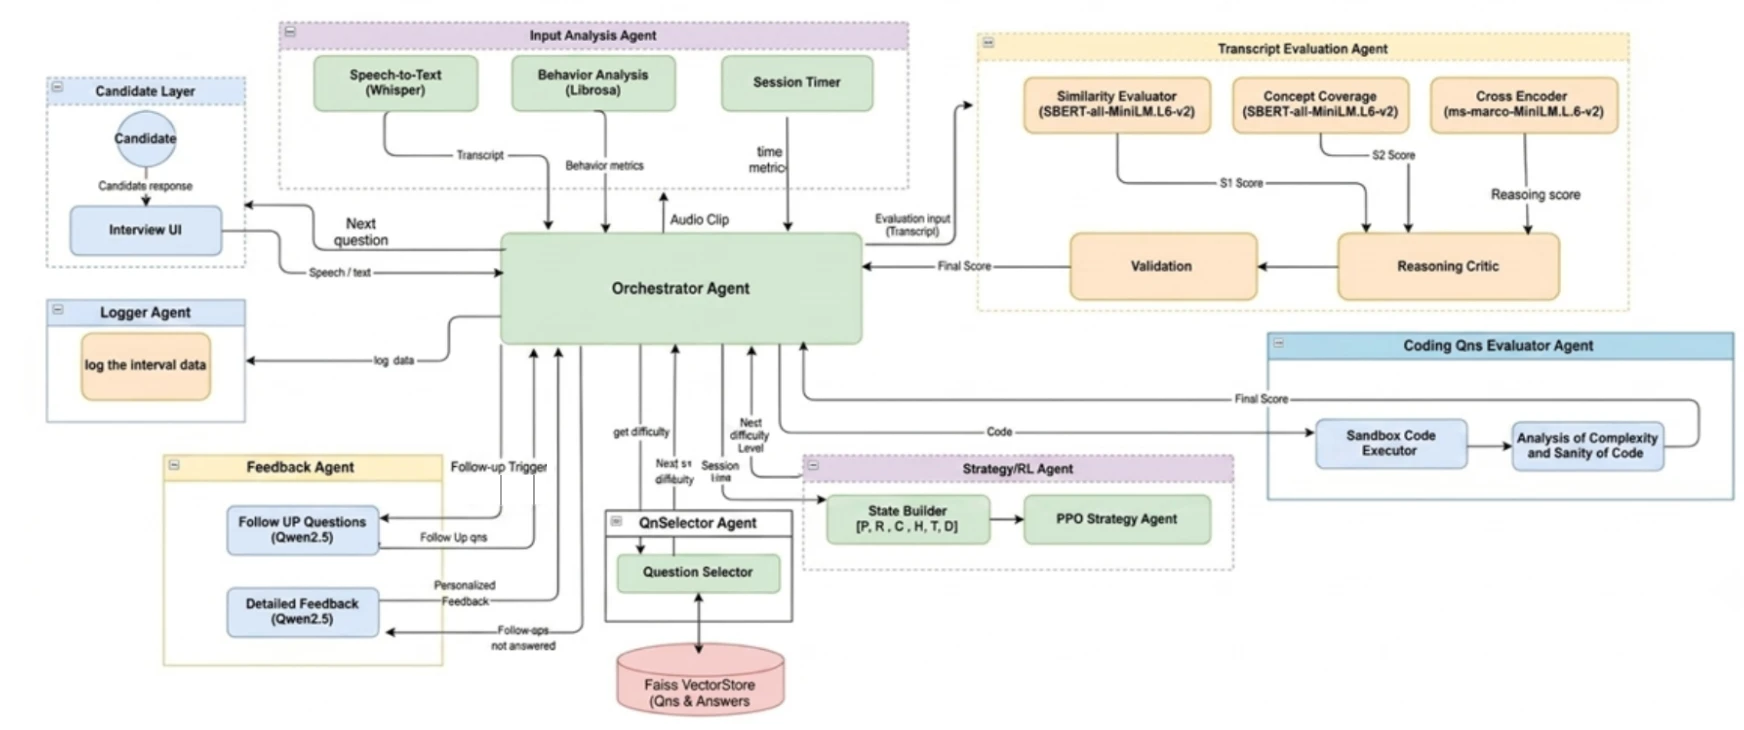
\includegraphics[width=\linewidth]{fig_architecture.png}
\caption{End-to-end flow of the interview application, from the first question shown to the candidate to the final score, feedback, and log. The Orchestrator Agent is the hub, the only writer of session state. The bounded-authority layer studied here (Strategy and Coaching agents, coordinator, arbitrator, guardrails) operates inside the orchestrator between the final score and the commit and is not drawn separately.}
\label{fig:arch}
\end{figure}

\textbf{Specialized Agent Roles and Private State.} Table~\ref{tab:authority} lists what each agent may propose and may not do. Under least privilege \cite{saltzer1975}, neither agent has state-write privileges; each receives an immutable, validated observation and returns a typed proposal. They are rule- and ledger-based, not LLM-driven: a compact design with private persistent state, pro-active proposals, and a communication channel, the properties of weak agency \cite{wooldridge1995} that the existing roles lacked.

\begin{table}[!htbp]
\caption{Authority matrix, generated from the enforcing code. Neither agent has state-write authority; the hub commits alone.}
\label{tab:authority}
\centering\scriptsize
\begin{tabular}{@{}L{1.3cm}L{2.9cm}L{2.4cm}L{2.9cm}L{1.8cm}@{}}
\toprule
Agent & May propose & Private state & Cannot & On invalid output\\
\midrule
Strategy & \texttt{difficulty\_action} (Easier, Same, or Harder); probe request (concept, kind); strategy mode & weakness ledger (per-concept miss counts, probe history, strategy trend) & write or overwrite any score; set a difficulty level directly; terminate the session; edit history; override hard constraints or guardrail overrides; call another agent & invalid, stale, low-confidence, or timed-out proposal is dropped; PPO proposal stands\\
\addlinespace
Coaching & feedback depth; hint/example flags; concepts to emphasize; remediation tag; tone & coaching history (hints and examples given, repeated misconceptions) & alter evaluator results or scores; cite concepts absent from evaluator evidence; request difficulty changes or follow-ups; terminate the session & invalid plan is dropped; the existing template feedback is used unchanged\\
\bottomrule
\end{tabular}
\end{table}

The matrix fixes what each component may \emph{propose} (typed, bounded fields) and what it may not \emph{commit}; the hub remains the only writer of authoritative state. The forbidden-key scan blocks proposals that smuggle a state field; stale-version checks prevent applying a proposal computed against an earlier state; the grounding check catches well-formed plans that credit a concept the evaluator never found. Schema validation addresses structural invalidity, not semantic correctness.

\textbf{Strategy Agent.} It maintains configured difficulty adaptation and tracks persistent weaknesses within the follow-up budget. Private state: per concept, the distinct turns in which it was missed or incorrect, later coverage, probes requested, and an exponential moving average (EMA) of scores. Rules, first match wins: \emph{recover} (a low current score with a low recent mean, or a weakness that survived its probes) $\to$ Easier; \emph{remediate} (a concept missed on two distinct turns and unresolved) $\to$ Same plus a probe request; \emph{stretch} (high current score and EMA, last three scores adequate, no open weakness) $\to$ Harder; otherwise \emph{steady} (Same). Thresholds are listed in Table~\ref{tab:prov}. Non-steady proposals carry confidence $\min(0.95,\,0.5+0.1n)$ for $n$ cited evidence items (a documented heuristic, not a calibrated probability); \emph{steady} proposals carry 0.45, below the arbitration threshold $\tau=0.6$, so the PPO action stands unless the ledger supports a change.

\textbf{Coaching Agent.} It chooses how to coach after an evaluated answer. Private state: concept miss counts and the hints and examples already given. Decisions: up to two concepts to emphasize, whether to give a hint or an example, feedback depth, tone, and a remediation tag; a Strategy peer message modifies the plan (\emph{recover}: detailed and encouraging; \emph{stretch}: brief; \emph{remediate}: remediation tag on the probed concept). A deterministic renderer applies the plan to the existing feedback and raises if a protected evaluator field would change.

\textbf{Communication and State Ownership.} Every observation, proposal, and decision is a typed object (unknown fields, NaN, and out-of-range values rejected). The coordinator records each call with session, turn, sender, recipient, state version, and provenance, and every accept, reject, or modify outcome with a reason code. Optimistic concurrency uses a state version that counts committed turns: a proposal whose version, turn, or session differs from the hub's is stale and dropped, and a second answer from the same agent for the same version is a duplicate and dropped.

\section{Orchestration, Arbitration and Validation}
\textbf{Difficulty precedence} (deterministic code, evaluated by ablation rather than assumed optimal), in order:
\begin{enumerate}\setlength{\itemsep}{0pt}\setlength{\topsep}{2pt}
\item hard constraints (infrastructure failure forces Same; levels stay in $[1,5]$);
\item the guardrail layer, applied last to whichever candidate was selected, wins whenever a rule fires;
\item a validated Strategy proposal with confidence $c\ge\tau$ and cited evidence supersedes the PPO action, recorded as a \emph{conflict};
\item the PPO action, or the labeled non-RL heuristic when PPO is unavailable.
\end{enumerate}
A proposal that cannot take effect at the bounds is recorded as \emph{modified}. \textbf{Probe precedence}, in order:
\begin{enumerate}\setlength{\itemsep}{0pt}\setlength{\topsep}{2pt}
\item the hard cap of two consecutive follow-ups;
\item a Strategy probe whose concept appeared in the evaluator's evidence earlier in the session and whose confidence satisfies $c\ge\tau$ (it may add a probe the thresholds would not trigger, or retarget the default one);
\item the hub's original threshold rule.
\end{enumerate}
The retargeted concept is passed to the template follow-up generator; the LLM prompt is not changed. Table~\ref{tab:trace} follows one recorded turn through these steps; in Step 5 rule G1 (overload protection: a low score at medium difficulty selects Easier) fires and selects the same Easier action as the Strategy candidate, so the guardrail layer retains it.

\begin{table}[!htbp]
\caption{One recorded turn (REPLAY; first replay cluster, original question order, condition $M_1$; state version 6). Rows are decision-record entries tagged by layer (P: proposal, C: control/admission, A: authoritative); a contrasting turn (version 5) is last.}
\label{tab:trace}
\centering\footnotesize
\begin{tabular}{@{}L{2.9cm}cL{4.3cm}L{3.3cm}@{}}
\toprule
Step (component) & L. & Content of the decision record & Recorded outcome\\
\midrule
1 Strategy proposal & P/C & Schema, forbidden-key, version, and grounding checks pass & accepted, \emph{valid}\\
2 Coaching proposal & P/C & Same checks; plan with depth \emph{detailed} & accepted, \emph{valid plan}\\
3 Arbitration & C & Strategy proposes Easier with confidence $\ge\tau$ and cited evidence & accepted, \emph{validated proposal}\\
4 PPO baseline & P & Proposed Same & rejected, \emph{superseded by Strategy} (a conflict)\\
5 Guardrail & C & Candidate Easier from Strategy; rule G1 (overload protection) fires and selects Easier & Easier accepted\\
6 Probe decision & C & Hub default rule & probe accepted, \emph{default policy}\\
7 Commit & A & The hub alone writes the level change and increments the state version & version $6\to7$\\
\addlinespace
Contrast, version 5 & C & Strategy proposes Same (\emph{steady}); PPO proposes Harder & Strategy rejected, \emph{low confidence} ($0.45<\tau=0.60$); PPO accepted, \emph{default policy}\\
\bottomrule
\end{tabular}
\end{table}

\textbf{PPO integration.} PPO keeps its role and its 6-D state and 3-action definitions; the policy was trained once and frozen before the multi-agent evaluation (Sect.~\ref{sec:method}), without hyperparameter search or result-based checkpoint selection. Its action is one input to arbitration; the agents never see it before proposing, and we make no claim that they improve PPO.

\textbf{Guardrails.} The deployed hub uses an inline copy of the rule layer that differs from the training environment's module; a configuration key selects the deployed (\emph{legacy inline}) or \emph{canonical} implementation, and both are reported. On a synthetic grid (39,930 points, hesitation $=1-$ acoustic confidence) the two disagree on 4,728 points (11.8\%); this is a property of the grid, not a deployment frequency.

\textbf{Proposal Validation.} Before any proposal reaches arbitration, the coordinator executes four sequential checks: (1) strict schema validation; (2) recursive scanning against 18 forbidden state keys; (3) optimistic concurrency verification against the hub's committed turn version; and (4) concept evidence grounding. If an agent raises an unhandled exception or exceeds its timeout (2\,s in XA and XC, 150\,ms in XB), its proposal is dropped and the hub proceeds with the default policy; a per-agent circuit breaker opens after two consecutive failures with a 60\,s cooldown.

\section{Experimental Methodology}\label{sec:method}
This section describes the dataset, the conditions, the experiments, the parameter provenance, and the statistics.
\textbf{Evaluation Environment and Replay Dataset.} All experiments run via deterministic replay through the real orchestrator hub, with the evaluator (the Transcript Evaluation Agent of Fig.~\ref{fig:arch}) replaced by recorded outputs. The data are 64 constructed (authored) answers to eight technical-interview questions, scored once by the production evaluator; the 64 payloads were recorded and replayed, and the evaluator is not re-run. The answers are authored, not an external public benchmark; the replay uses recorded evaluator outputs and no human ratings (reference scores from three raters appear only in the exploratory evaluator analysis below). Each replay cluster is the $k$-th recorded answer set across the eight questions ($k=1,\ldots,8$); follow-up probes reuse the payload recorded for the root concept. This is a deterministic replay study of fixed stimuli and recorded evaluator outputs, not an evaluation of closed-loop adaptation to human candidates. Evidence classes are labeled by experiment: REPLAY (XA, XC, and the split versus unified comparison), FAULT-INJECTED (XB), SYNTHETIC (the authored feedback probes of XD and the guardrail state-grid analysis), and SIMULATED (PPO training against a synthetic candidate model, evidence about the policy, not about real candidates). Replay sessions combine the 8 clusters with 20 question orders (seeds 0--19; seed 0 is the original order, seeds 1--19 apply a seeded shuffle per cluster), yielding $N=160$ sessions per condition. These sessions are not independent: they reuse the same 8 clusters, which we treat as the independent structural units in cluster-aware analyses. No live generative LLM is invoked; the LLM gateway is stubbed as down and deterministic template renderers produce text. Per-turn latency was timed in-process with a monotonic wall-clock timer. Pooled p50 and p95 timings are descriptive; because replay hardware and operating system were not recorded, absolute values are not portable benchmarks, latency effects are interpreted through paired condition differences, and no cluster-level interval was computed for latency.

\textbf{Baseline and Ablation Matrix.} Experiment XA addresses RQ1 (chiefly $M_1$ versus $B_0$) and, through its ablations, RQ3 (arbitration) and RQ4 (authority and grounding safeguards); RQ2 is addressed by the split-versus-unified comparison, RQ3 additionally by XC, and RQ4 by XB and XD. XA evaluates the following conditions across the identical 160 replay sessions:
\begin{itemize}\setlength{\itemsep}{0pt}\setlength{\topsep}{2pt}
\item $B_0$: frozen single-controller workflow without agents, PPO active, inline guardrails. $B_7$: $B_0$ with PPO unavailable (deterministic rule fallback). $B_{0c}$: $B_0$ with the canonical guardrail module.
\item $M_1$: full multi-agent system (Strategy and Coaching agents, peer messaging, arbitration with $\tau=0.6$). $M_7$: $M_1$ with PPO disabled (paired with $B_7$). $M_{1c}$: $M_1$ with canonical guardrails.
\item $M_2$: Strategy Agent ablated (Coaching and the coordination layer remain active). $M_3$: Coaching Agent ablated (Strategy remains active). $M_6$: Strategy-to-Coaching peer messaging disabled.
\item $M_4$: arbitration and downstream admission-control bypass, so raw Strategy proposals are admitted without confidence-threshold, evidence-grounding, step-bound, or guardrail-layer checks; because it removes several mechanisms at once, it is not a pure arbitration-only ablation. $M_5$: grounding verification ablated (Coaching plans accepted without concept-evidence checks). $M_8$: authority enforcement ablated (score authority verification bypassed before proposal admission).
\end{itemize}

\textbf{Framework for Evaluating Agent Specialization (RQ2).} We contrast (1) the specialized architecture ($\Msplit$), the two-agent configuration $M_1$ with separate state ledgers and explicit peer messaging, and (2) a unified architecture ($\Munified$), a monolithic agent with a joint session ledger that synthesizes difficulty actions, follow-up probes, and coaching plans in a single dispatch. Both receive identical observations, questions, thresholds, and arbitration rules. Outcomes are the decision agreement rate ($P(\mathrm{Decision}_{\mathrm{unified}}=\mathrm{Decision}_{\mathrm{split}})$), with difficulty-action and follow-up probe agreement as components, per-turn dispatch and serialization latency, and architectural state encapsulation (schema and ledger boundaries).

\textbf{Threshold Decomposition (Experiment XC).} Because the bypassed condition ($M_4$) simultaneously removes the confidence threshold, evidence verification, and one-step limits, it cannot isolate which mechanism prevents oscillation collapse. XC provides the narrower isolation of the confidence-threshold mechanism: it sweeps $\tau\in\{0.0,0.5,0.6,0.7,0.8,0.9\}$ across the same 160 replay sessions while holding all other guardrail boundaries and evidence checks active. Five predictions (C1--C5, Table~\ref{tab:pred}) were pre-specified in the internal protocol record before any XC run, with $\tau=0.6$ fixed in advance (internal protocol registration, not external preregistration). The value $\tau=0.60$ is a selected operating point, not a tuned optimum; it was not tuned against replay outcomes.

\textbf{Fault Injection and Circuit Breaker (Experiment XB).} To test whether bounded authority contains component failures (RQ4), constructed faults were injected into the real agents during replay. Strategy faults were crash, timeout, malformed output, forbidden state key, stale version, NaN confidence, and adversarial-valid (a well-formed, authorized proposal opposing the evidence); Coaching faults were crash, malformed output, stale version, and ungrounded (a valid plan emphasizing a concept absent from the evaluator evidence). Adversarial-valid and ungrounded faults fired on every call; the others fired with probability 0.3 per agent call (seeded). One pre-specified, exploratory prediction (B6, Table~\ref{tab:pred}) concerned the per-agent circuit breaker opening at least once in at least 80\% of full-path crash, malformed, stale, and NaN-confidence sessions. Each fault was crossed with four variants (full path, authority check removed, arbitration removed, grounding check removed) over 40 sessions per cell (8 clusters $\times$ 5 order seeds) with a 150\,ms agent timeout. A fault counted as contained only if the session completed, committed scores equaled the evaluator output, and every difficulty transition was valid; guardrail bypass, ungrounded-concept leakage, and breaker opening were counted per session. Each variant removes a mechanism and then injects the fault it guards against, so results show the necessity of a mechanism for the tested property, not general fault tolerance.

\textbf{Grounding Probe (Experiment XD).} Separately from the proposal-level concept-grounding check, the deployed lexical feedback validator was probed with authored (synthetic) feedback texts; no LLM was involved. For each of the 64 recorded evaluator payloads, seven constructed feedback categories were checked (for example faithful text, a score leak, and truncated paraphrase credit, which credits a concept in paraphrase without supporting evidence). Placeholder concept texts were relabeled uniquely to remove an evidence artifact, and a category was counted only for payloads where it could be constructed.

\textbf{Provenance and Reproducibility.} Table~\ref{tab:prov} records how each parameter was chosen and whether it changed after replay results were observed; no parameter has a logged tuning procedure and nothing was tuned on replay results (the evaluator concept threshold and dampening were fixed on an earlier pilot, before replay, and the pilot records are not recoverable). Every condition uses one frozen PPO checkpoint, the deployed runtime policy (seed 123, SHA-256 prefix \texttt{2ab8d514}), trained once for a nominal 100,000 steps (100,352 executed) with Stable-Baselines3 PPO and frozen before the multi-agent evaluation; no result from any other checkpoint is used. Training was SIMULATED: a single synthetic candidate (fixed skill $\approx0.6$, one persona, skill constant over time) generated scores, confidence, and hesitation for the six-dimensional state, with actions Easier, Same, and Harder. The candidate noise generator was not seeded, so training is not bit-reproducible; the training seed fixes the policy initialization, action sampling, and the environment's own random draws. The reward largely imitates a hand-coded rule oracle (agreement weight 0.60, outcome change 0.30, shaping 0.10), consistent with the small effect of disabling PPO (A9). Training used horizon $T=15$ with continuous difficulty steps, whereas the pipeline uses integer levels 1--5, which limits transferability; no multi-candidate, human-candidate, or online learning is involved.

The cross-encoder is called through the sentence-transformers \texttt{predict} interface; its single-output result $r$ is mapped to $R=\mathrm{clip}((r-0.20)/0.70,\,0,\,1)$, after which the concept threshold (0.30) and the dampening of $S_2$ by 0.6 when $R\le0.30$ apply. The library's default activation for a single-label head is a sigmoid, but the saved model configuration was not retained for confirmation, so we do not characterize $r$ further. The checkpoint was trained under Windows 11, Python 3.12.7, Stable-Baselines3 2.7.1, PyTorch 2.2.2 (CPU), NumPy 1.26.4, and Gymnasium 0.29.1 (recorded in the checkpoint file); the replay used Python 3.11 with unrecorded, unrecoverable package versions (including those of the evaluator-related libraries), and replay hardware and operating system were not recorded.

\textbf{Evaluator dependence (exploratory).} Replay outcomes depend on recorded evaluator outputs, and evaluator validity is not evaluated here. A separate exploratory analysis on the 64 constructed answers found a Spearman correlation of $\rho=0.4832$ between the cross-encoder signal $R$ and the reference score, $\rho=0.3812$ for the deployed composite, and $\rho=0.4897$ for a word-count-only baseline. $R$ was strongly associated with answer length ($\rho=0.6594$, 95\% CI $[0.457,0.831]$), and the length-controlled partial correlation of $R$ with the reference score was $0.2434$ (95\% CI $[-0.008,0.507]$), so a length-independent contribution is not established; this neither shows that $R$ carries no information nor validates the evaluator. The reference scores are internal scores from three raters, and rater provenance and ethics documentation are incomplete, so the analysis is exploratory; the replay itself does not use them. The $0.15/0.35/0.50$ weights are design-time weights, not tuned on the current replay study; $R$ carries half of the composite weight and is associated with length in the exploratory analysis. Weight selection will be tested on development data with length-robust baselines (P5, Sect.~\ref{sec:limits}).

\begin{table}[!htbp]
\caption{Parameter provenance. No parameter has a logged tuning procedure; ``design-time'' means chosen before the experiments without a recorded selection study. The last column rests on the protocol record; protocol identifiers are local commits.}
\label{tab:prov}
\centering\scriptsize
\begin{tabular}{@{}L{1.5cm}L{3.7cm}L{2.8cm}L{1.2cm}L{2.2cm}@{}}
\toprule
Parameter & Value & How chosen & Fixed before replay? & Changed after observing replay?\\
\midrule
Strategy rules & persistent after 2 misses; at most 2 probes; recover score $0.35$; stretch score $0.8$, EMA $0.7$ ($\alpha=0.5$), last three $\ge0.6$ & design-time constants; no tuning record & yes & No\\
Coaching rules & hint if score $<0.6$ and $<2$ hints; depth detailed $<0.4$, brief $\ge0.85$; $\le2$ emphasized concepts & design-time constants; no tuning record & yes & No\\
Confidence & $\min(0.95,0.5+0.1n)$; \emph{steady} 0.45 & design-time heuristic; uncalibrated & yes & No\\
$\tau$ & 0.60 & design-time; fixed before XC, not tuned & yes & No\\
XC sweep & $\tau\in\{0,0.5,0.6,0.7,0.8,0.9\}$ & designed after inspecting XA and XB & no (post-hoc design) & Not applicable (post-hoc design)\\
Guardrails & levels 1--5; step $\le1$; six rules & inherited from the earlier controller; deployed and canonical copies & yes & No (inherited)\\
Agent timeout & 2\,s (XA, XC); 150\,ms (XB) & experiment configuration & yes & No\\
Breaker & 2 consecutive failures, 60\,s cooldown & implementation default & yes & No\\
PPO checkpoint & seed 123; nominal 100,000 steps (100,352 executed); SHA-256 prefix \texttt{2ab8d514} & trained once, not selected on replay & yes & No (inherited checkpoint)\\
PPO training settings & lr $3\times10^{-4}$, 2,048 steps/rollout, batch 64, 10 epochs, $\gamma=0.99$, clip 0.2, GAE 0.95 & library-style defaults in the training script; no search & yes & No (inherited checkpoint)\\
Evaluator weights & 0.15/0.35/0.50 ($S_1$, $S_2^{\mathrm{eff}}$, $R$) & design-time; no tuning artifact survives & yes (recorded outputs) & No\\
Evaluator thresholds & concept threshold 0.30; dampening 0.6 if $R\le0.30$; $R=(r-0.20)/0.70$ clipped & concept threshold and dampening fixed on an earlier pilot, before replay; pilot records and remaining details not recoverable & yes (recorded outputs) & No\\
Fault rates & 0.3 per call (seeded); adversarial and ungrounded faults on every call & fixed in the protocol & yes & No\\
Replay design & 8 clusters $\times$ order seeds 0--19 (seed 0 original); cluster bootstrap $B=10{,}000$, seed 20270101 & fixed in the protocol & yes & No\\
\bottomrule
\end{tabular}
\end{table}

\textbf{Statistical Methodology.} For session-level point estimates and paired differences, we compute standard non-parametric percentile bootstrap intervals with $B=10{,}000$ resamples. For bounded completion, transition, and invariant proportions, we report exact Clopper--Pearson binomial confidence intervals \cite{clopper1934}. To account for the 8-cluster dependency, we implement a cluster bootstrap over the 8 underlying replay clusters following Field and Welsh \cite{field2007} ($B=10{,}000$), resampling entire replay clusters with replacement. We also report a leave-one-cluster-out (LOCO) sensitivity analysis. All intervals are descriptive; no significance tests or $p$-values are computed.

\begin{table}[!htbp]
\caption{Replay ablation summary (160 sessions per condition; mean per session unless noted). compl./auth./trans.: sessions completing, keeping committed scores authoritative, and preserving valid transitions. chg./rev.: level changes and reversals; agr.: fraction of final actions equal to the PPO action (below 1 in $B_0$ because guardrails override PPO); gfire: guardrail overrides; strat.: decisions where Strategy was the final action source; byp.: sessions with guardrail bypass; p50/p95: pooled per-turn latency (ms); calls: agent calls per session. $M_4$ is the arbitration and downstream admission-control bypass.}
\label{tab:ablation}
\centering\scriptsize
\begin{tabular}{@{}lccccrrrrcccc@{}}
\toprule
Cond. & compl. & auth. & trans. & chg. & rev. & agr. & gfire & strat. & byp. & p50 & p95 & calls\\
\midrule
$B_0$ & 160&160&160& 15.119& 11.744& 0.626& 9.588& 0.0& 0& 0.546& 2.056& --\\
$B_7$ & 160&160&160& 2.675& 1.256& --& 3.831& 0.0& 0& 0.463& 1.059& --\\
$B_{0c}$ & 160&160&160& 15.119& 11.744& 0.626& 9.588& 0.0& 0& 0.553& 2.004& --\\
$M_1$ & 160&160&160& 12.45& 9.869& 0.4& 6.838& 6.669& 0& 1.589& 4.411& 47.68\\
$M_2$ & 160&160&160& 15.119& 11.744& 0.626& 9.588& 0.0& 0& 1.218& 3.513& 23.25\\
$M_3$ & 160&160&160& 12.45& 9.869& 0.4& 6.838& 6.669& 0& 1.118& 3.189& 23.84\\
$M_4$ & 160&160&160& 2.225& 1.0& 0.014& 0.0& 19.619& 3& 1.573& 4.357& 47.68\\
$M_5$ & 160&160&160& 12.45& 9.869& 0.4& 6.838& 6.669& 0& 1.581& 4.553& 47.68\\
$M_6$ & 160&160&160& 12.45& 9.869& 0.4& 6.838& 6.669& 0& 1.592& 4.46& 47.68\\
$M_8$ & 160&160&160& 12.45& 9.869& 0.4& 6.838& 6.669& 0& 1.575& 4.35& 47.68\\
$M_7$ & 160&160&160& 2.706& 1.312& --& 3.812& 9.037& 0& 1.502& 2.968& 47.68\\
$M_{1c}$ & 160&160&160& 12.45& 9.869& 0.4& 6.838& 6.669& 0& 1.573& 4.534& 47.68\\
\bottomrule
\end{tabular}
\end{table}

\begin{table}[!htbp]
\caption{Paired $M_1-B_0$ differences over the 160 sessions. Naive intervals resample sessions and are descriptive only; cluster intervals resample the 8 replay clusters ($B=10{,}000$) and are the primary inference. LOCO: range of the mean difference over the eight leave-one-cluster-out analyses (number of 95\% intervals excluding zero); Same sign: clusters whose own difference shares the sign of the point estimate. Latency was not analyzed by cluster. Paired path, level-change, reversal, and agreement differences are zero for $M_2$ vs.\ $B_0$, $M_3,M_5,M_6,M_8$ vs.\ $M_1$, $B_{0c}$ vs.\ $B_0$ and $M_{1c}$ vs.\ $M_1$.}
\label{tab:paired}
\centering\scriptsize
\resizebox{\linewidth}{!}{\begin{tabular}{@{}lccccc@{}}
\toprule
$M_1-B_0$ (per session) & Point & Naive 95\% CI & Cluster 95\% CI & LOCO range (CI excl.\ 0) & Same sign\\
\midrule
Level changes & $-2.669$ & $[-3.188,-2.131]$ & $[-4.50,-0.24]$ & $[-3.76,-2.20]$ (1/8) & 7/8\\
Reversals & $-1.875$ & $[-2.275,-1.462]$ & $[-3.12,-0.27]$ & $[-2.57,-1.52]$ (4/8) & 7/8\\
PPO agreement & $-0.226$ & $[-0.244,-0.208]$ & $[-0.284,-0.170]$ & $[-0.244,-0.203]$ (8/8) & 8/8\\
Follow-up (probe) turns & $+0.588$ & $[+0.338,+0.850]$ & $[0.000,+1.763]$ & $[0.000,+0.671]$ (0/8) & 1/8\\
Median turn latency (ms) & $+1.043$ & $[+1.000,+1.079]$ & not computed & not computed & --\\
\bottomrule
\end{tabular}}
\end{table}

\section{Results}\label{sec:results}
All results derive from deterministic REPLAY of recorded evaluator outputs unless noted, and sessions within a condition are dependent across question orders (Sect.~\ref{sec:method}). Table~\ref{tab:pred} lists every pre-specified prediction with its status; three were contradicted (A9, A10, B6).

\textbf{Coordination: Trajectory Divergence and Reduced Level Changes (RQ1).} Enabling the agent layer ($M_1$) altered the difficulty trajectory relative to the frozen baseline ($B_0$) in all 160 replay sessions (A7), with fewer level changes and reversals and lower agreement with the PPO action (Tables~\ref{tab:ablation} and \ref{tab:paired}). Strategy remained the final action source in 6.669 decisions per session after guardrails (strat.\ in Table~\ref{tab:ablation}).

\textbf{Cluster Dependence and Fragility.} The effects differ in robustness. Omitting replay cluster $k=1$ shifts the level-change difference to $-3.76$ (CI $[-4.81,-2.78]$), whereas omitting any other cluster makes the 95\% interval include zero; the sign is shared by 7 of the 8 clusters. The cluster interval rests on only 8 clusters and is approximate, so we report the direction as consistent and the magnitude as uncertain. Reversals are similar (LOCO intervals exclude zero in 4 of 8), and PPO agreement is the most stable (8 of 8). The probe effect is the most fragile: the $+0.59$ turns per session arise in only 1 of 8 clusters ($k=1$), so it cannot be generalized.

\textbf{Proposals and Overhead.} The Strategy Agent generated 3,814 proposals (including 1,274 steady proposals at confidence 0.45) and no stretch proposals (0): the replayed candidates never met the sustained-performance criteria. The layer raised pooled median per-turn latency from 0.546\,ms to 1.589\,ms ($+1.04$\,ms) and the 95th percentile from 2.056\,ms to 4.411\,ms, with 47.7 agent calls per session.

\textbf{Arbitration and Admission Control (RQ3).} Disabling the Strategy Agent ($M_2$) reproduced the baseline difficulty, score, and question trajectories in 160 of 160 sessions (A4), so Strategy is the only channel through which the layer changes difficulty. In the arbitration and downstream admission-control bypass ($M_4$), trajectories collapsed (2.225 level changes per session, PPO agreement 0.014) with guardrail bypass in 3 of 160 sessions. Because $M_4$ removes several mechanisms at once, Experiment XC varies only the confidence threshold $\tau$ (Table~\ref{tab:xc}).

\begin{table}[!htbp]
\caption{Experiment XC (REPLAY, 160 sessions per row, mean per session): only the confidence threshold $\tau$ varies; evidence checks and guardrails remain active. Column definitions as in Table~\ref{tab:ablation} (strat. precedes gfire here).}
\label{tab:xc}
\centering\footnotesize
\begin{tabular}{@{}rrrrrrr@{}}
\toprule
$\tau$ & chg. & rev. & agr. & strat. & gfire & byp.\\
\midrule
0.0 & 2.225 & 1.000 & 0.014 & 16.075 & 3.544 & 0\\
0.5 & 12.450 & 9.869 & 0.400 & 6.669 & 6.838 & 0\\
0.6 & 12.450 & 9.869 & 0.400 & 6.669 & 6.838 & 0\\
0.7 & 12.450 & 9.869 & 0.400 & 6.669 & 6.838 & 0\\
0.8 & 12.450 & 9.819 & 0.404 & 6.594 & 6.863 & 0\\
0.9 & 15.119 & 11.744 & 0.626 & 0.000 & 9.588 & 0\\
\bottomrule
\end{tabular}
\end{table}

At $\tau=0.0$ the trajectory collapses toward the bypassed regime (Table~\ref{tab:xc}) with zero bypass, because steady proposals (confidence 0.45) override PPO on most RL decisions (16.1 of 19.6 per session). Behavior is flat across $\tau\in[0.5,0.7]$ because realized confidences take the discrete values 0.70 and 0.80; at $\tau=0.9$ the threshold exceeds every realized confidence, so Strategy cannot supersede PPO and trajectories revert to $B_0$. Because the confidence values are few and structured, the sweep cannot resolve finer threshold effects, and $\tau=0.60$ sits inside a stable plateau rather than at a demonstrated optimum. All five pre-specified XC predictions were supported. Disabling grounding ($M_5$) or the Strategy-to-Coaching message ($M_6$) left trajectories identical to $M_1$ (A5), and disabling PPO ($M_7$) altered only 4 of 160 sessions (2.5\%), contradicting A9, because the Strategy heuristic usually reaches the same action as the non-RL fallback. Canonical guardrails changed no path (0/160, A10) because the divergent grid states (extreme hesitation or low voice confidence) were never reached under neutral replay acoustics.

\begin{table}[!htbp]
\caption{Pre-specified predictions and status (A: Experiment XA, B: XB, C: XC; internal protocol record, not external preregistration). Ceiling rows hold in every condition and do not discriminate between conditions. Three predictions were contradicted (A9, A10, B6).}
\label{tab:pred}
\centering\scriptsize
\begin{tabular}{@{}L{0.9cm}L{5.2cm}L{3.4cm}L{1.9cm}@{}}
\toprule
ID & Predicted property & Observed & Status \\
\midrule
A1--A3 & completion 100\%; committed scores equal evaluator output; levels in $[1,5]$, steps $\le1$ & 160/160 in every condition & Supported \\
A4 & $M_2$ reproduces $B_0$ paths & 160/160 sessions & Supported \\
A5 & $M_3,M_5,M_6,M_8$ reproduce $M_1$ & identical paths & Supported \\
A6 & $M_4$ bypass in $\ge1$ session, $M_1$ none & 3/160 vs 0/160 & Supported \\
A7 & $M_1\ne B_0$ in $\ge50\%$ of sessions & 160/160 & Supported \\
A8 & median latency $M_1-B_0<50$\,ms & $+1.043$\,ms & Supported \\
A9 & $M_7\ne B_7$ in $\ge50\%$ of sessions & 4/160 (2.5\%) & \textbf{Contradicted} \\
A10 & canonical guardrails change $\ge1$ path & 0/160 & \textbf{Contradicted} \\
B1 & full path: contained, no bypass or leak & all cells 40/40, 0, 0 & Supported \\
B2 & forbidden key: authority vs schema rejection & 152 vs 152; 40/40 contained & Supported \\
B3 & adversarial: bypass without arbitration & 38/40 vs 0/40 & Supported \\
B4 & ungrounded: leak without grounding & 40/40 vs 0/40 & Supported \\
B5 & timeout raises p95 by $\ge100$\,ms & 154.4 vs 4.4\,ms & Supported \\
B6 & breaker opens in $\ge80\%$ of sessions & 29/40 (72.5\%) & \textbf{Contradicted} \\
C1 & $\tau=0$: agreement $<0.10$, changes $<5.0$, no bypass & 0.014, 2.225, 0 & Supported \\
C2 & $\tau=0.6$ reproduces $M_1$ & identical & Supported \\
C3 & $\tau=0.5$ equals $\tau=0.6$ & identical & Supported \\
C4 & Strategy decisions non-increasing in $\tau$ & 6.669, 6.669, 6.594, 0 & Supported \\
C5 & $\tau=0.9$ below half of $\tau=0.6$ & 0 vs 6.669 & Supported \\
\bottomrule
\end{tabular}
\end{table}

\textbf{Specialization: Trajectory Invariance under Functional Decomposition (RQ2).} Removing the Coaching Agent ($M_3$) gave trajectories identical to $M_1$ in all 160 sessions (A5). This follows from the topology (the coaching plan has no difficulty-control field and communication runs only from Strategy to Coaching), so $M_3\equiv M_1$ is true by construction. The split-versus-unified comparison is likewise a consistency check, not evidence of a benefit. A unified controller that re-implements the same rule set with a joint ledger produced identical normalized decisions (difficulty action, mode, confidence, probe concept, and coaching plan fields) on all 1,280 matched open-loop turns, so $P(\mathrm{Decision}_{\mathrm{unified}}=\mathrm{Decision}_{\mathrm{split}})=1.0$, with identical difficulty and probe paths. Dispatch latency was 0.0440\,ms (split) versus 0.0401\,ms (unified, $-8.9\%$) and validating two typed models took 0.0092\,ms versus 0.0038\,ms for one ($-58.7\%$); these are descriptive single-run measurements, distinct from the end-to-end $+1.04$\,ms overhead of $M_1$ over $B_0$. No behavioral advantage of specialization was observed in this controlled setting.

\textbf{Bounded Authority: Invariant Enforcement and Containment (RQ4).} Every condition completed all 160 sessions, kept committed scores equal to the recorded evaluator output, and enforced bounds in $[1,5]$ with steps of at most one level (A1--A3; exact Clopper--Pearson 95\% lower bound for 160/160: 0.977 \cite{clopper1934}); this is completion and containment under the specified protocol, not general fault tolerance. Under full bounded authority ($M_1$) and throughout XC, guardrail bypass stayed at zero. In fault injection (Table~\ref{tab:xb}; 40 sessions per cell), adversarial-valid proposals bypassed guardrails in 38 of 40 sessions without arbitration (95\% CI $[0.831,0.994]$) and in 0 of 40 with it (95\% CI $[0.000,0.088]$), and ungrounded concepts were emphasized in 40 of 40 sessions without the grounding check and in 0 of 40 with it. The circuit breaker opened in 29 of 40 sessions (72.5\%, 95\% CI $[0.561,0.854]$), below the pre-specified 80\% expectation (B6). Timing-out proposals gave a p95 turn latency of 154.4\,ms (each call bounded by the 150\,ms timeout). In the lexical probe (XD), unsupported paraphrased credit was accepted in 57 of 57 applicable authored cases (95\% CI $[0.937,1.000]$): the validator enforces a lexical evidence contract, not semantic verification.

Containment is a ceiling result in every cell; discrimination comes only from the removed-mechanism variants, and removing the authority check changed no outcome because schema validation alone contained the forbidden-key faults (B2 in Table~\ref{tab:pred}; Table~\ref{tab:threat}). Removing arbitration produced bypass in 34 of 40 sessions in the non-adversarial Strategy fault cells, which is not comparable with the 3 of 160 sessions of $M_4$ in XA: there the faulted calls open the breaker, the Strategy proposal is absent on many decisions (449 of 938 Strategy calls in the full-path crash cell were rejected as breaker-open), and with arbitration removed the guardrail layer is skipped, so the unguarded base action is committed. Bypass counts correlate negatively with Strategy-sourced decisions per session (Spearman $\rho=-0.62$ over the 240 such sessions); this mechanism reading is descriptive, and the correlation does not establish causality.

\begin{table}[!htbp]
\caption{Fault injection (FAULT-INJECTED, 40 sessions per cell). Contained: the session completed, committed scores equaled evaluator output, and all transitions were valid. Bypass: sessions with guardrail bypass; Leak: sessions with ungrounded-concept emphasis; Breaker: sessions in which the circuit breaker opened. $^\dagger$See text; not comparable with XA $M_4$.}
\label{tab:xb}
\centering\scriptsize
\begin{tabular}{@{}L{4.0cm}lccccc@{}}
\toprule
Fault (injected calls per cell) & Variant & Sess. & Contained & Bypass & Leak & Breaker\\
\midrule
Strategy crash, timeout, malformed, stale, NaN, forbidden key (152 each; identical rows) & full path & 40&40&0&0&29\\
 & no authority check & 40&40&0&0&29\\
 & no arbitration & 40&40&34$^\dagger$&0&29\\
 & no grounding & 40&40&0&0&29\\
\midrule
Strategy adversarial-valid (930) & full path & 40&40&0&0&0\\
 & no authority check & 40&40&0&0&0\\
 & no arbitration & 40&40&38&0&0\\
 & no grounding & 40&40&0&0&0\\
\midrule
Coaching crash, malformed, stale (154 each; identical rows) & full path & 40&40&0&0&29\\
 & no authority check & 40&40&0&0&29\\
 & no arbitration & 40&40&1&0&29\\
 & no grounding & 40&40&0&0&29\\
\midrule
Coaching ungrounded (950) & full path & 40&40&0&0&0\\
 & no authority check & 40&40&0&0&0\\
 & no arbitration & 40&40&1&0&0\\
 & no grounding & 40&40&0&40&0\\
\bottomrule
\end{tabular}
\end{table}

\begin{table}[!htbp]
\caption{Threat model and safeguard matrix. Columns are mechanisms (Sch.: schema; Aut.: authority; Ver.: version; Gnd.: grounding; Arb.: arbitration; Brk.: breaker). R: rejects the threat in the logged reason codes; N: removal changed the outcome; O: removal tested, no change; P: the proposal passes the check; --: not applicable. No single safeguard covers every fault class; only authority, arbitration, and grounding were ablated.}
\label{tab:threat}
\centering\scriptsize
\begin{tabular}{@{}L{3.1cm}ccccccL{3.1cm}@{}}
\toprule
Threat (source) & Sch. & Aut. & Ver. & Gnd. & Arb. & Brk. & Tested result \\
\midrule
Forbidden key, unauthorized write (faulty agent) & R & R,O & -- & -- & -- & R & contained; schema alone suffices \\
Malformed, NaN, or stale proposal (faulty agent) & R & -- & R & -- & -- & R & contained \\
Ungrounded coaching emphasis (faulty agent) & -- & -- & -- & R,N & O & -- & 40/40 leak without grounding \\
Adversarial-valid Strategy proposal (well-formed, evidence-opposing) & P & O & P & O & N & -- & 38/40 bypass without arbitration \\
Repeatedly failing agent & -- & -- & -- & -- & -- & R & breaker opened in 29/40; not ablated \\
Slow proposal & -- & -- & -- & -- & -- & R & p95 154.4\,ms; sessions complete \\
Invalid transition magnitude & -- & -- & -- & -- & -- & -- & step-bound guardrail; bounds held in all cells \\
Wrong but lexically grounded content & -- & -- & -- & P & -- & -- & not contained (57/57 accepted) \\
\bottomrule
\end{tabular}
\end{table}

\section{Discussion}
\textbf{Admission of agent proposals changes behavior; role splitting preserved it.} Under the tested replay conditions, introducing the agent layer altered the difficulty trajectory relative to the frozen baseline ($B_0$), whereas reorganizing identical responsibilities into specialized versus unified components did not alter matched per-turn decisions. This is consistent with the change arising from the introduction and admission of auxiliary recommendations, while specialization reorganizes responsibility and state boundaries. The split-versus-unified result is a consistency check on a re-implementation of the same rules, not evidence that specialization has or lacks value in general.

\textbf{Arbitration as the control point.} Ablating Strategy ($M_2$) reproduced the baseline, whereas removing Coaching ($M_3$) or the peer message ($M_6$) left the trajectory unchanged: Strategy influenced difficulty only through the arbitration/admission pathway, since neither agent has state-write authority, and Coaching has no authority over difficulty. Removing arbitration and downstream admission control ($M_4$) collapsed the trajectory, and the threshold sweep indicated that $\tau$ controls proposal admission. $M_1$ versus $B_0$ adds the Strategy rules, the confidence gate, and the agent structure together; the ablations ($M_2$, $M_4$, XC) place the change in the Strategy proposal and its admission, but the study cannot separate the added rules from an agent layer. PPO has little influence here: disabling it changed 4 of 160 sessions (A9).

\textbf{Lower volatility is not better adaptation.} $M_1$ showed fewer level changes and reversals than $B_0$ (Table~\ref{tab:paired}), but removing arbitration gave an even flatter trajectory while abandoning PPO alignment and allowing bypass. Stability and adaptation are distinct objectives, and stability is a systems metric, not a pedagogical criterion.

\textbf{Authority and containment.} Fault injection supports a narrow containment claim under the tested fault model: schema validation, forbidden-key scanning, and version checks intercepted malformed, unauthorized, and stale proposals; grounding addressed unsupported attribution; the breaker handled repeated failures; and arbitration contained adversarial-valid proposals. This is a layered safeguard picture, not a proof of general safety, and structural or lexical validation does not establish semantic correctness.

\textbf{Design lessons from this case study.} (i) Separate proposal generation from authoritative state mutation (Tables~\ref{tab:authority} and \ref{tab:xb}). (ii) In the tested setting, central arbitration was more behaviorally consequential than role splitting (Tables~\ref{tab:paired} and \ref{tab:ablation}). (iii) Safety controls should operate downstream of proposal generation, and overlapping safeguards cannot be told apart without ablation (Tables~\ref{tab:xb}, \ref{tab:threat}, \ref{tab:ablation}). (iv) Different fault classes need different safeguards (Tables~\ref{tab:xb} and \ref{tab:threat}). (v) Negative specialization results are useful: organization alone produced no behavioral benefit here (Sect.~\ref{sec:results}). 

\section{Limitations and Threats to Validity}\label{sec:limits}
Table~\ref{tab:limits} lists the limitations.

\begin{table}[!htbp]
\caption{Limitations, their effect on claims, and planned future work (P1--P8, Sect.~\ref{sec:limits}).}
\label{tab:limits}
\centering\scriptsize
\begin{tabular}{@{}L{5.0cm}L{4.4cm}L{2.2cm}@{}}
\toprule
Limitation & Effect on claims & Future work\\
\midrule
Deterministic replay of 64 constructed answers (8 clusters, 20 orders); no human ratings in the replay; pre-computed candidate responses; no closed-loop adaptation & Metrics describe decision dynamics, not learning or pedagogical efficacy; level-change effect is cluster-sensitive & P2, P8\\
One frozen PPO checkpoint trained on one synthetic constant-skill candidate with unseeded noise and a rule-imitating reward; simulator horizon and continuous difficulty differ from the integer-level pipeline & Coordination comparison is checkpoint-specific; no PPO benefit for real candidates & P1, P2\\
Split-versus-unified agreement holds for deterministic rule- and ledger-based agents under open-loop replay & No equivalence claim for stochastic agents, live LLMs, or closed-loop settings & P4\\
No acoustic waveforms; stretch branch and guardrail-disagreement region unexercised & Harder branch and acoustic effects untested & P2\\
Evaluator outputs fixed; evaluator not externally validated; exploratory length association & Evaluator errors propagate into decisions; weights unvalidated & P5\\
$\tau=0.60$ is a design-time operating point; confidence is an uncalibrated discrete heuristic; XC designed after XA/XB; design-time parameters (Table~\ref{tab:prov}); local protocol commits & Thresholds not claimed optimal; no external timestamps & P6\\
Replay package versions (including evaluator libraries), hardware, and operating system unrecorded & Limits exact reproduction; latency not portable & --\\
No fairness, adverse-impact, or psychometric analysis; communication-confidence signal unvalidated; accent and recording-condition bias unevaluated & No fairness claims & P8\\
Fault injection covers tested defects only; lexical grounding accepted unsupported paraphrase (57/57) & No universal fault tolerance or semantic-correctness guarantee & P3, P7\\
\bottomrule
\end{tabular}
\end{table}

\textbf{Data and ethics.} No human participants were involved, no live interviews were conducted, and the replay corpus contains no personal data. No institutional ethics review was sought or is claimed; any future human evaluation will require approval. In real deployment, voice and answer data can constitute personal data, and the communication-confidence signal is not a validated psychological measure; accent, speech-pattern, or recording-condition differences could introduce bias, and any deployment would require explicit consent, a retention policy, and appropriate governance. None of these properties was evaluated here.

\textbf{Artifact availability and reproducibility.} Code, configurations, seeds, aggregate results, and table-generation scripts exist in the authors' repository and are not publicly released at submission; the cross-encoder weights have incomplete provenance and are not claimed to be redistributable. Replay inputs, clusters, seeds, conditions, checkpoint identity, protocol values, bootstrap parameters, fault rates, and analysis definitions are documented here; replay package versions (including evaluator libraries), hardware, and operating system are unrecoverable, which limits exact environment reproduction.

\textbf{Planned extensions.} Planned extensions (protocols only, not run): P1 stronger baselines, P2 closed-loop simulator, P3 semantic grounding, P4 LLM-backed Strategy Agent, P5 evaluator validation, P6 continuous confidence, P7 property-based authority tests, P8 small human study (ethics approval required).

\section{Conclusion}
This study asked whether any change in the decisions of an adaptive technical-interview system stems from specialization or from coordination and arbitration. Across 160 deterministic replay sessions per condition, adding the agent layer with confidence-gated arbitration altered difficulty trajectories relative to the frozen single-policy baseline, although the magnitude was sensitive to the eight replay clusters. A matched open-loop comparison of the specialized and unified designs produced identical decisions on all 1,280 turns, a consistency check on the re-implementation: under the tested replay conditions, role splitting preserved behavior. Bounded-authority mechanisms gave mechanism-specific containment of the evaluated injected faults.

The evaluation does not establish human-candidate efficacy, pedagogical benefit, online candidate learning, equivalence for live stochastic LLM agents, general semantic correctness, universal fault tolerance, or general superiority of specialization or PPO. Specialization structures responsibility and private state, whereas coordination and arbitration determine which proposal becomes authoritative. Future work should test these boundaries across policy checkpoints, human candidates, and generative multi-agent architectures (Sect.~\ref{sec:limits}).

\let\oldthebibliography\thebibliography
\let\endoldthebibliography\endthebibliography
\renewenvironment{thebibliography}[1]{%
  \begin{oldthebibliography}{#1}%
    \setlength{\itemsep}{0pt}%
    \setlength{\parsep}{0pt}%
    \emergencystretch=4em%
}{%
  \end{oldthebibliography}%
}
\bibliographystyle{splncs04}
\bibliography{refs}
\end{document}
